\chapter{Calcolo delle Variazioni}
\section{Preliminari}
Il calcolo delle variazioni si occupa dell'ottimizzazione di funzioni $ F : X \to \R $, dove $X$ è un insieme di funzioni.\\
In questo capitolo varranno considerati univocamente funzionali integrali del tipo
\[
	\begin{array}{rcc}
		F: X & \to & \R \\
		x & \to & \int_{a}^b f(t,x(t), x'(t))\integrald{t}
	\end{array}
\]
eventualmente soggetti a vincoli sui valori $x(a)$ e $x(b)$ o sul valore di un integrale del tipo $\int_a^b \varphi(x(t))\integrald{t}$.\\
\begin{note}
	Un funzionale è una qualsiasi funzione definita su un insieme di funzioni $ X $ (spazio funzionale) con valori in $ \R $ o $ \C $.
	Molto informalmente, possiamo dire che un funzionale è una funzione avente come variabili indipendenti delle funzioni.
	Si tratta infatti non più di analisi matematica, ma di analisi funzionale.
\end{note}
Dove:
\[f: \intervalclose{a}{b}\times \R ^n\times \R ^n \to \R\]
\[X=\brackets{x\in \cntclass{1}(\intervalclose{a}{b}; \R^n)\text{ : }x(a)=x_a, x(b)=x_b },\text{ con }x_a,x_b\in \R ^n\]
con $ \intervalclose{a}{b} \in \R $ un intervallo.
\proposition
Sia $f\in \cntclass{1}(A\times \R ; \R )$ con $A \subseteq \R ^n$\\
Se
\[ F: \R \times \R \times A \to \R \]
\[ x \to \int_{\alpha}^\beta f(x,t)\integrald{t} \]
Allora:
\[ F\in \cntclass{1}\]
\[ \partial_\alpha F(\alpha,\beta,x)=-f(x,\alpha)\]
\[ \partial_\beta F(\alpha,\beta,x)=f(x,\beta)\]
\[ \nabla_x F(\alpha,\beta,x)=\int_{\alpha}^{\beta}\nabla_xf(x,t)\integrald{t}\]
\begin{proof}
	L'integrale di una funzione $ f \in \cntclass{1} $ continua ad appartenere a $ \cntclass{1} $ (già dimostrato).\\
	Sia $ \varphi(x(t),t) $ la primitiva di $ f(x(t),t) $ rispetto a $ t $,
	ovvero $ \partial_t \varphi(x(t),t) = \varphi'(x(t),t)*x'(t) = f(x(t),t) $.\\
	Formalizziamo anzitutto la soluzione generica di un integrale definito come:\\
	\[F(\alpha,\beta,x) = \varphi(x(\beta),\beta) - \varphi(x(\alpha),\alpha) \]\\
	Si risolvano dunque i singoli integrali con le derivate parziali, partendo da $ \alpha $:\\
	\begin{align*}
		\partial_\alpha F(\alpha,\beta,x) &= \partial_\alpha \left[\varphi(x(\beta),\beta) - \varphi(x(\alpha),\alpha)\right]\\
		&= \partial_\alpha \varphi(x(\beta),\beta) - \partial_\alpha \varphi(x(\alpha),\alpha)\\
		&= 0 - f(x(\alpha),\alpha)\\
		&= - f(x(\alpha),\alpha)
	\end{align*}
	seguendo con $ \beta $:\\
	\begin{align*}
		\partial_\beta F(\alpha,\beta,x) &= \partial_\beta \left[\varphi(x(\beta),\beta) - \partial_\beta \varphi(x(\alpha),\alpha)\right]\\
		&= \partial_\beta \varphi(x(\beta),\beta) - \partial_\beta \varphi(x(\alpha),\alpha)\\
		&= f(x(\beta),\beta) - 0\\
		&= f(x(\beta),\beta)
	\end{align*}
	poiché $ \alpha $ e $ \beta $ non dipendono da x, non vi è alcun calcolo da svolgere
	(il gradiente per linearità può star dentro o fuori dal simbolo di integrale).
\end{proof}
\begin{note}
	Si ricordi \textbf{SEMPRE} che l'integrale è un operatore, come lo possono essere il prodotto o la somma e dunque si opera su esso
	senza considerarlo più speciale o diverso.
\end{note}
\begin{note}
	La proposizione appena esposta non è strettamente inerente a questo capitolo. Tuttavia, è riportata in quanto esplicita il risultato di un integrale
	data la derivazione parziale rispetto ad uno degli estremi di integrazione o rispetto alle variabili di integrazione ($ t $ escluso). 
\end{note}

\newpage
\section{L'Equazione di Eulero}
\begin{lemma}[Lemma Fondamentale del Calcolo delle Variazioni]
	\index{Lemma!Fondamentale del Calcolo delle Variazioni}
	\label{lemma:fond_calc_var}
	Sia $f\in \cntclass{0}(\left[0,1\right]; \R )$ t.c. $\forall v\in \cntclass{0}(\left[0,1\right]; \R )$
	con $v(0)=v(1)=0$ si abbia
	\[\int_0^1 f(x)v(x)\integrald{x}=0\]
	Allora $f(x)\equiv 0 \forall x \in \left[0,1\right]$ 
	\begin{proof}
		Ipotizziamo per assurdo che $ \exists x_0 \in \left[0,1\right] $ t.c. $ f(x_0) > 0$.\\
		Allora, poiché $ f \in \cntclass{0} $, esiste un intervallo $ \left] a,b \right[ \in \left[0,1\right] $ t.c. $ f(x) > f(x_0)/2$.\\
		Definiamo (sotto rappresentata graficamente):
		\[
			\begin{array}{rcc}
				v: \left[0,1 \right] & \to & \R\\
				x & \to &
				\begin{cases}
					0 & \text{se } x < a\\
					2 \frac{x-a}{b-a} & \text{se } x \in \left[ a, (a+b)/2 \right]\\
					2 \frac{b-x}{b-a} & \text{se } x \in \left[ (a+b)/2, b  \right]\\
					0 & \text{se } x > b
				\end{cases}
			\end{array}
		\]
		\begin{center}
			\begin{tikzpicture}[scale=4]
				\draw[->] (0,0) -- (1.2,0) node[anchor=north west] {$x$};
				\draw[->] (0,0) -- (0,1.2) node[anchor=south east] {$y$};
				\node[below] at (0.0,0) {0};
				\node[below] at (0.35,0) {$a$};
				\node[below] at (0.35,0.5) {$f(x_0)/2$};
				\node[below] at (0.5,0) {$x_0$};
				\node[below] at (0.65,0) {$b$};
				\node[below] at (1,0) {1};
				\clip (0,0) rectangle (1,1);
				\draw[domain=0:0.2,smooth,red,variable=\x] plot ({\x},{0});
				\draw[domain=0.2:0.5,smooth,red,variable=\x] plot ({\x},{(1/0.3)*\x-(0.2/0.3)});
				\draw[domain=0.5:0.8,smooth,red,variable=\x] plot ({\x},{-(1/0.3)*\x+(0.8/0.3)});
				\draw[domain=0.8:1,smooth,red,variable=\x] plot ({\x},{0});
				\draw[domain=0.35:0.65,smooth,dashed,blue,variable=\x] plot ({\x},{0.5});
			\end{tikzpicture}
		\end{center}
		Allora
		\begin{align*}
			\int_0^1f(x)v(x)\integrald{x} &\geq \int_a^bf(x)v(x)\integrald{x}\\
			&\geq\frac{f(x_0)}{2}\int_a^bv(x)\integrald{x}\\
			&=\frac{f(x_0)}{2}\frac{b-a}{2}>0\\
			&=\frac{(b-a)f(x_0)}{4}\\
			&> 0
		\end{align*}
		con $ f(x_0) > 0 $ dall'ipotesi assurda che implica la negazione dell'ipotesi, dunque l'assurdo.
	\end{proof}
\end{lemma}
\corollary
\label{coro:gen_fond_calc_var}
Sia $f\in \cntclass{0}(\left[a,b\right]; \R ^n)$ tale che $\forall v\in \cntclass{0}(\left[a,b\right]; \R ^n)$
con $v(0)=v(1)=0$ si abbia $\int_0^1f(x)\bullet v(x)\integrald{x}=0$ allora $f(x)\equiv \vec{0}$ $\forall x\in \left[0,1\right]$.
\begin{proof}
	Per questa dimostrazione si osservano componente per componente.\\
	$\forall i=1,2,\ldots,n$ scelgo $v_j(x)=\left\{\begin{matrix}0&&j\ne i\\v_i(x)&&j=i \end{matrix}\right.$\\
	A questo punto applico il lemma fondamentale alla componente $i$-esima $f_i$ di $f$.
\end{proof}
\corollary
Sia $f\in \cntclass{0}(\left[a,b\right]; \R )$ e $k\in\mathbb{N}$ tale che $\forall v\in \cntclass{k}(\left[a,b\right]; \R ^n)$ con $v(0)=v(1)=0$
si abbia $\int_0^1f(x)v(x)\integrald{x}=0$ allora $f(x)\equiv \vec{0}$ $\forall x\in \left[0,1\right]$.
\begin{proof}
	\'E sempre lo stesso lemma con l'aggiunta che la funzione $v$ sia di classe $\cntclass{k}$.\\
	\begin{center}
		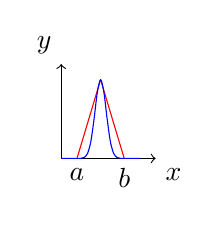
\begin{tikzpicture}[scale=1]
			\draw[->] (0,0) -- (1.2,0) node[anchor=north west] {$x$};
			\draw[->] (0,0) -- (0,1.2) node[anchor=south east] {$y$};
			\node[below] at (0.2,0) {$a$};
			\node[below] at (0.8,0) {$b$};
			\clip (0,0) rectangle (1,1);
			\draw[domain=0:0.2,smooth,red,variable=\x] plot ({\x},{0});
			\draw[domain=0.2:0.5,smooth,red,variable=\x] plot ({\x},{(1/0.3)*\x-(0.2/0.3)});
			\draw[domain=0.5:0.8,smooth,red,variable=\x] plot ({\x},{-(1/0.3)*\x+(0.8/0.3)});
			\draw[domain=0.8:1,smooth,red,variable=\x] plot ({\x},{0});
			\draw[domain=0:1,smooth,blue,variable=\x] plot ({\x},{ e^(-((\x-0.5)*10)^2) });
		\end{tikzpicture}
	\end{center}
	Se si chiama $v$ la funzione blu e $u$ la funzione rossa.\\
	Si osservi che $v$ è una funzione più regolare di $u$.\\
	Tutte le funzioni $ v \in \cntclass{k} $ a loro volta sono t.c $ v \in \cntclass{0} $.
	Dunque le ipotesi di \ref{lemma:fond_calc_var} sono soddisfatte ed è dimostrato.
\end{proof}
\observation
Il Teorema seguente è concettualmente analogo al Teorema di Fermat nel capitolo sulla differenziabilità.
Infatti, esso fornisce una condizione \textbf{NECESSARIA MA NON SUFFICIENTE} al primo ordine per punti di minimo o massimo locali.
\begin{theorem}[EQUAZIONE DI EULERO]
	\index{Teorema!Equazione di Eulero}
	\label{teo:equazione_eulero}
	Sia $f\in \cntclass{2}\left(\left[ 0,1 \right]\times \R^n\times \R^n; \R \right)$ e fissati i valori $x_0, x_1 \in \R^n$.\\
	Sia $ X=\brackets{x\in \cntclass{1}\left(\left[ 0,1 \right]; \R^n\right): x(0) = x_0, x(1) = x_1} $.\\
	Siano:
	\[
		\begin{array}{ccc}
			F: \cntclass{1}\left(\left[ 0,1 \right]; \R^n\right) &\to & \R\\
			x &\to & \int_0^1 f(t, x(t), x'(t))\integrald{t}
		\end{array}
	\]
	Se la funzione $ x_\ast $ è tale che
	\[ x_\ast\in X \text{ è t.c. } F(x_\ast)=\min\brackets{F(x):x\in X }\]
	Allora
	\[\partial_xf(t,x_\ast(t), x_\ast'(t))-\frac{d}{\integrald{t}}\partial_{ x'}f(t,x_\ast(t), x_\ast'(t))=0 \]
	Quest'ultima equzione è detta equazione di Eulero-Lagrange del Funzionale $F$ o a volte detta variazione prima del funzionale $F$.
	\'E un sistema di $n$ equazioni differenziali ordinarie del secondo ordine nella funzione incognita $x_\ast$.\\
	Analogamente esiste un enunciato per i punti di massimo.
	\begin{proof}
		Sia $x$ di minimo per $F$. Si definisca una funzione qualunque
		\[ v \in \cntclass{1}\left(\left[ 0,1 \right]; \R^n\right) \text{ con } v(0) = v(1) = 0, \]
		$ \forall h \in \R, h < \varepsilon $, con $\varepsilon$ sufficientemente piccolo (come nella definizione di limite), si ha
		$ \left( x + hv \right) \in X $. Data
		\begin{align*}
			\varphi(h) &= F\left( x + hv \right)\\
			&= \int_0^1 f(t, x + hv, x' + h\dot{v})\integrald{t}
		\end{align*}
		si ha un minimo in $ h = 0 $, in quanto $ F(x + 0) = F(x) $ il quale è di minimo per com'è stato scelto.\\
		$\varphi$ è derivabile rispetto ad $h$, dunque, se si considera la derivata direzionale lungo
		$ \vec{v} = \begin{bmatrix}
			v \\
			\dot{v}
		\end{bmatrix} $,
		e il $ \nabla F(x) = \begin{bmatrix}
			\int_0^1 \left(\frac{\partial f}{\partial x}(t, x + hv, x' + h\dot{v})\right)\integrald{t} &
			\int_0^1 \left(\frac{\partial f}{\partial x'}(t, x + hv, x' + h\dot{v})\right)\integrald{t}
		\end{bmatrix}$ si ha:
		\begin{align*}
			\varphi'(h) &= \nabla F(x + h\vec{v}) \cdot \vec{v}\\
			&= \int_0^1 \left(\frac{\partial f}{\partial x}(t, x + hv, x' + h\dot{v}) v \right)\integrald{t}\\
			&+ \int_0^1 \left(\frac{\partial f}{\partial x'}(t, x + hv, x' + h\dot{v}) \dot{v} \right)\integrald{t}\\
			\varphi'(0) &= \int_0^1 \left(\frac{\partial f}{\partial x}(t, x, x') v + \frac{\partial f}{\partial x'}(t, x, x') \dot{v} \right)\integrald{t}
		\end{align*}
		Si consideri ora solo il secondo addendo e lo si integri per parti,
		considerando $\dot{v}$ come la funzione da integrare e la derivata parziale come la funzione da derivare:
		\begin{align*}
			\int_0^1 \frac{\partial f}{\partial x'}(t, x, x') \dot{v} \integrald{t}
			&= 0 - 0 -\int_0^1 \frac{d}{dt}\frac{\partial f}{\partial x}(t, x, x') v \integrald{t}\\
			&= -\int_0^1 \frac{d}{dt}\frac{\partial f}{\partial x'}(t, x, x') v \integrald{t}
		\end{align*}
		e quindi sostituendo il risultato appena ottenuto con il secondo addendo
		\[ \varphi'(0) = \int_0^1 \left(\frac{\partial f}{\partial x}(t, x, x') - \frac{d}{dt}\frac{\partial f}{\partial x'}(t, x, x') \right)v \integrald{t} \]
		Ricordando che $\varphi(0)$ è un punto singolare, e dunque $\varphi'(0) = 0$, sono dunque soddisfatte le ipotesi di \ref{lemma:fond_calc_var} e si ha
		\[ \frac{\partial f}{\partial x}(t, x, x') - \frac{d}{dt}\frac{\partial f}{\partial x'}(t, x, x') = 0 \]
		ovvero la tesi.
	\end{proof}
\end{theorem}

\section{Geodetica}
Il problema della Geodetica è il seguente: dati due punti nello spazio, determinare la più breve curva di classe $ \cntclass{1} $ che li congiunge.\\
Nel piano le geodetiche giacciono sempre su rette, nelle sfere sugli archi di cerchio massimo.\\
A breve sarà più chiaro, ma anche in questo caso il concetto di distanza risulterà fondamentale.\\
Si parta da alcune definizioni e concetti preliminari.
\definition
Sia $ I \in \R $ un intervallo. Allora
\[
	\begin{gathered}
		\text{curva } \gamma\\
		\bydef\\
		\gamma: I \to R^m
	\end{gathered}
\]
\observation
$\gamma(I)$ si chiama supporto della curva, ed è certamente connesso.(una funzione continua manda intervalli connessi in spazi connessi).
\definition
Sia $\gamma : \intervalclose{a}{b} \to \R^n$ una curva, sia $ p = \brackets{ t_k }_k^n $ una partizione dell'intervallo $ \intervalclose{a}{b} $
ovvero un insieme finito di punti t.c. $ a = t_0 < t_1 < t_2 < \ldots < t_n = b $, allora
\[
	\begin{gathered}
		\text{lunghezza della curva}\\
		\bydef\\
		l(\gamma)=\sup\brackets{\sum\limits_{i=1}^{N}d\left(\gamma(t_i), \gamma(t_{i-1})\right): N \in p,|p|>1}
	\end{gathered}
\]
ovvero si prende la curva originale e la si approssima con una curva spezzata i cui vertici appartengono alla curva originale.
Più è grande $ p $, più sarà accurata.\\
\definition
Una curva $\gamma : \intervalclose{a}{b} \to \R^n$ si dice rettificabile $\bydef l(\gamma)<+\infty$, ovvero la lunghezza della curva è finita.
\proposition
\label{prop:lunghezza_curva_integrale}
Se $\gamma\in \cntclass{1}(\intervalclose{a}{b}; \R ^n)\implies l(\gamma)=\int_a^b\norm{\gamma'(t)}\integrald{t}$.
\observation
Se $\gamma$ è la traiettoria di un punto materiale, allora $l(\gamma)$ è lo spazio che si percorre e $\norm{\gamma'}$ è la norma della velocità istantanea.\\
Infatti, lo spazio percorso è l'integrale della velocità valutato tra due istanti di tempo $a$ e $b$ (estremi di integrazione).
\doublespacing
\par
Si prenda ora come \textbf{caso di studio il \textcolor{red}{piano}} (anziché la sfera o altre figure).\\
Si fissi l'origine in uno dei due punti, sia $A(x_A,y_A)$ l'altro. Posto il funzionale
\[
	X = \brackets{
		\varphi \in \cntclass{1}\left(\left[ 0,1 \right]; \R^2\right) : 
		\begin{cases}
			\varphi'(t) \neq 0 \forall t \in \left[ 0,1 \right]\\
			\varphi(0) = \left( 0,0 \right)\\
			\varphi(1) = \left( x_A,y_A \right)
		\end{cases}
	}
\]
data la lunghezza di una curva $l(\varphi)$, il problema consiste nel determinare il punto di minimo di $l$ su $X$, ovvero
\[ l(\varphi) = \min\brackets{l(\varphi) : \varphi \in X}. \]
Avendo preso come caso di studio il piano si ha $n = 2$,
dunque le componenti di $\varphi(t)$ sono $ \left(x(t),y(t)\right) $.\\
La lunghezza della curva definita in \ref{prop:lunghezza_curva_integrale}, data la definizione di $X$ in questo caso di studio diviene
\[ l(\varphi)=\int_0^1 \norm{\varphi'(t)}\integrald{t} \]
e dunque $f$ dipende solo da $x' \text{ e } y'$. Ipotizzando di utilizzare la norma euclidea si ha dunque
\[ f(t; x, t; x', y') = \sqrt{x'^2 + y'^2}. \]
Si applichi l'Equazione di Eulero all'ultima equazione:
\[
	\begin{cases}
		\frac{\partial f}{\partial x}(t, x, x') - \frac{d}{dt}\frac{\partial f}{\partial x'}(t, x, x') =
		\partial_x \sqrt{x'^2 + y'^2} - \frac{d}{dt}\partial_{x'} \sqrt{x'^2 + y'^2} =
		0 - \frac{d}{dt} \frac{x'}{\sqrt{x'^2 + y'^2}}
		\\
		\frac{\partial f}{\partial x}(t, x, x') - \frac{d}{dt}\frac{\partial f}{\partial x'}(t, x, x') =
		\partial_y \sqrt{x'^2 + y'^2} - \frac{d}{dt}\partial_{y'} \sqrt{x'^2 + y'^2} =
		0 - \frac{d}{dt} \frac{y'}{\sqrt{x'^2 + y'^2}}
	\end{cases}
\]
e dunque, inserendo il lato destro delle Equazioni di Eulero, si ha
\[
	\begin{cases}
		\frac{d}{dt} \frac{x'}{\sqrt{x'^2 + y'^2}} = 0\\
		\frac{d}{dt} \frac{y'}{\sqrt{x'^2 + y'^2}} = 0
	\end{cases}
\]
Sapendo che l'unica funzione con derivata sempre nulla è la funzione costante si ha
\[
	\begin{cases}
		\frac{x'}{\sqrt{x'^2 + y'^2}} = \text{costante}
		\\
		\frac{y'}{\sqrt{x'^2 + y'^2}} = \text{costante}
	\end{cases}
\]
Quindi, la curva che rende minima $l$ ha il suo versore tangente \textbf{sempre} costante. L'unica funzione che soddisfa tale condizione è la retta.
\begin{note}
	Si ricorda che le derivate prime (in questo caso $x', y'$) sono le tangenti nel punto.\\
	Il vettore in questione è un versore in quanto viene normalizzato dal termine al denominatore.
\end{note}

\section{La Brachistocrona}
Il problema della Brachistocrona è il seguente: determinare la curva congiungente due punti assegnati lungo cui sia minimo il tempo di caduta
di un oggetto puntiforme dotato di massa soggetto alla sola forza di gravità.\\
\par
Si utilizzerà come sistema di riferimento l'asse $x$ orizzontale e $y$ verticale orientato verso il basso e l'origine nel punto di partenza.\\
Sia $(\bar{x}, \bar{y})$ il punto finale.\\
Sia $ y = y(x) $ l'equazione della curva cercata.\\
Sia $ x \in \left[0, \bar{x}\right]$, ovvero appartenente a un intervallo.\\
Per il Principio di Conservazione dell'Energia si ha, ad una data quota $y$, il modulo della velocità è pari a $ \sqrt{2gy(x)} $.\\
Lo spazio infinitesimo percorso sulla curva, dato un tratto infinitesimo percorso sull'asse $x$,
è dato da $ \integrald{s} = \sqrt{1 + (y')^2} \integrald{x} $.
Tale valore è meglio intelligibile se visto come modulo della quantità di spazio percorso sulla curva $y$ dato uno spostamento sull'asse $x$
ovvero $ \frac{\integrald{s}}{\integrald{x}} = \sqrt{(x')^2 + (y')^2} $, ottenuto dividendo per $\integrald{x} $ con un leggero abuso di notazione.
Si constata che $x$, in quanto variabile indipendente è esattamente la bisettrice fra il primo e terzo quadrante e dunque $ x' = 1 $
dunque si ha $ \frac{\integrald{s}}{\integrald{x}} = \sqrt{1 + (y')^2} $.\\
Noto che la velocità è spazio su tempo, il tempo infinitesimo di percorrenza è $ \integrald{t} = \frac{\sqrt{1 + (y')^2}}{\sqrt{2gy(x)}} \integrald{x} $.\\
Il tempo totale per compiere il tragitto è dunque
\[ T(y) = \int_0^{\bar{x}} \sqrt{\frac{1 + (y')^2}{2gy(x)} \integrald{x}. \]
Si consideri il funzionale
\[ F(x) = \int_{t_0}^{t_1} \varphi(x) \cdot \sqrt{1 + (x')^2 \integrald{x} \]
e la sostituzione
\[ \psi(x') = \sqrt{1 + (x')^2 \]
l'Equazione di Eulero \ref{teo:equazione_eulero} corrispondente moltiplicando a destra e sinistra per $x'$
\[
	\begin{align*}
		x' \cdot \left(\frac{\partial f}{\partial x} - \frac{d}{dt}\frac{\partial f}{\partial x'}\right) &= 0\\
		x' \cdot \left[\varphi'(x)\psi(x') - \frac{d}{dt}\left(\varphi(x)\psi'(x')\right)\right] &= 0\\
		x' \cdot \left[\frac{d}{dt}\frac{\varphi(x)}{x'}\psi(x') - \frac{d}{dt}\left(\varphi(x)\psi'(x')\right)\right] &= 0\\
		\frac{d}{dt}\left[ \varphi(x)\psi(x') - x'\varphi(x)\psi'(x') \right] &= 0\\
		\frac{d}{dt}\left[ \varphi(x)(\psi(x') - x'\psi'(x')) \right] &= 0
	\end{align*}
\]
dato
\[
	\begin{align*}
		\psi(x') - x'\psi'(x') &= \sqrt{1 + (x')^2} - x' \frac{x'}{\sqrt{1 + (x')^2}}\\
		&= \sqrt{1 + (x')^2} - \frac{(x')^2}{\sqrt{1 + (x')^2}}\\
		&= \frac{1 + (x')^2 - (x')^2}{\sqrt{1 + (x')^2}}\\
		&= \frac{1}{\sqrt{1 + (x')^2}}
	\end{align*}
\]
e dunque sostituendo
\[
	\begin{align*}
		\frac{d}{dt}\left[ \varphi(x)\frac{1}{\sqrt{1 + (x')^2}} \right] &= 0\\
		\frac{d}{dt} \frac{\varphi(x)}{\sqrt{1 + (x')^2}} &= 0.
	\end{align*}
\]
L'equazione di Eulero per $T(y)$ nella forma appena individuata è
\[
	\begin{align*}
		\frac{d}{dx} \frac{1}{\sqrt{2gy} \cdot \sqrt{1 + (y')^2}} &= 0\\
		\frac{d}{dx} \frac{1}{\sqrt{2gy \cdot (1 + (y')^2)}} &= 0\\
	\end{align*}
\]
Sapendo che l'unica funzione con derivata sempre nulla è la funzione costante si ha
\[ \frac{1}{\sqrt{2gy \cdot (1 + (y')^2)}} &= k \]
\[ \sqrt{2gy \cdot (1 + (y')^2)} &= \frac{1}{k} \]
\[ 2gy \cdot (1 + (y')^2) &= \frac{1}{k^2} \]
\[ y \cdot (1 + (y')^2) &= \frac{1}{2gk^2} \]

\begin{note}
	Nei prossimi passaggi verranno usate diverse relazioni trigonometriche facilmente dimostrabili. Se non note, munirsi di formulario.
\end{note}

Sostituendo $ y' = \frac{dy}{dx} = \left[ \tan(\theta/2) \right]^{-1} $ si ottiene
\[ y \cdot (1 + \frac{1}{\tan^2(\theta/2)} ) = \frac{1}{2gk^2} \]
\[ y \cdot \frac{\tan^2(\theta/2) + 1}{\tan^2(\theta/2)} &= \frac{1}{2gk^2} \]
\[ y = \frac{1}{2gk^2} \cdot \frac{\tan^2(\theta/2)}{\tan^2(\theta/2) + 1} \]
\[ y = \frac{1}{2gk^2} \cdot \sin^2(\theta/2) \]
\[ y = \frac{1}{2gk^2} \cdot \sqrt{\frac{1 - \cos \theta}{2}} \sqrt{\frac{1 - \cos \theta}{2}} \]
\[ y = \frac{1}{2gk^2} \cdot \frac{1 - \cos \theta}{2} \]
\[ y = \frac{1}{4gk^2} \cdot \left(1 - \cos \theta\right) \]
la parametrizzazione rispetto a $x$ si ottiene considerando la funzione inversa di quella appena usata per effettuare la sostitituzione, ovvero
$ \frac{dx}{dy} = \tan(\theta/2) = \frac{1 - \cos \theta}{\sin \theta} $
\[ \frac{dy}{d\theta} = \frac{1}{4gk^2} \cdot \left(\sin \theta\right) \]
\[ \frac{dx}{dy} \frac{dy}{d\theta} = \frac{1 - \cos \theta}{\sin \theta} \frac{1}{4gk^2} \cdot \left(\sin \theta\right) \]
\[ \frac{dx}{d\theta} = \frac{1}{4gk^2} \cdot \left(1 - \cos \theta\right) \]
\[ x = \frac{1}{4gk^2} \cdot \left(\theta - \sin \theta\right) \]
e dunque, riassumendo, le equazioni parametriche sono
\[
	\begin{cases}
		x = \frac{1}{4gk^2} \cdot \left(\theta - \sin \theta\right)\\
		y = \frac{1}{4gk^2} \cdot \left(1 - \cos \theta\right)
	\end{cases}
\]
con $k$ determinata da $ y(\bar{x}) = \bar{y} $.\\
La curva trovata è un arco di Cicloide, ovvero una curva generata dalla rotazione di una circonferenza.\\
In questo caso il raggio corrisponde a $ r = \frac{1}{4gk^2} $.\\
\newpage
\begin{figure}[h]
	\caption{Una Cicloide}
	\centering
	\includegraphics[width=0.5\textwidth]{images/Cicloide.png}
\end{figure}
\begin{figure}[h]
	\caption{Brachistocrona fra due punti a diverse altezze (in rosso)}
	\centering
	\includegraphics[width=0.5\textwidth]{images/Brachistochrone.png}
\end{figure}
